\begin{figure}[htp]
\begin{center}

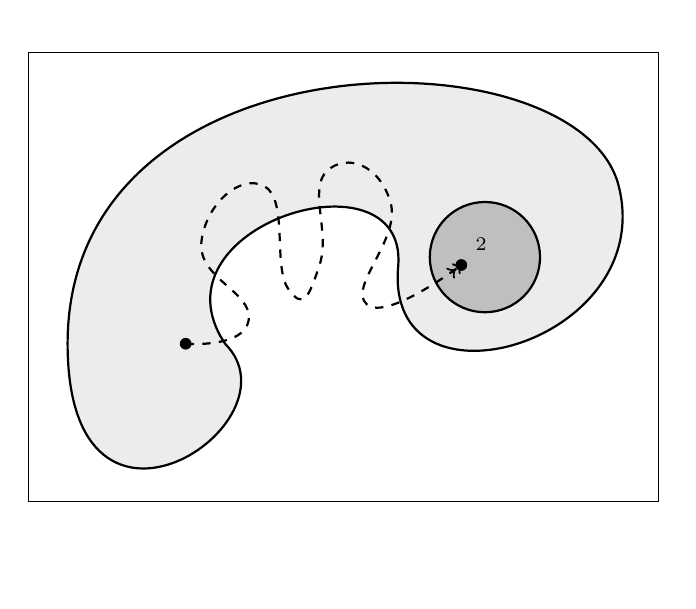
\begin{tikzpicture}

% help grid
\draw[draw] (-0.5,1) rectangle (7.5,6.7);
\node[label={below left:$\bbR$}] at (7.5,6.7) {};

%%% Bezier curves for bean shape %%%
\draw[thick, fill=gray!15] (0,3) .. controls (0,7) and (6.5,7)  ..  (7,5) .. controls (7.5,3) and (4,2) ..  (4.2,4) .. controls (4.3,5.5) and (1,4.5) .. (2,3).. controls (3,2) and (0,0) .. (0,3);
%% end bezier curves for bean shape %%%

% integer solution circle
\draw[thick, fill=gray!50] (5.3,4.1) circle (.7cm);
% point inside the circle
\node[inner sep = 1.5pt, black, circle, fill, label={above right:$\bbZ_2$}] at (5,4) (circP){};

% point inside bean
\node[inner sep = 1.5pt, black, circle, fill] at (1.5,3) (beanP) {};

% path from beanP to circP
%\draw[gray] (beanP) -- (2.3,3.3) -- (1.7,4.3) -- (2.5,5) -- (2.8,3.7) -- (3.2,4) -- (3.3,5.2) -- (4.1,4.8) -- (3.8,3.5) -- (circP);
\draw[dashed, thick, ->>] plot [smooth, tension=1] coordinates {(beanP) (2.3,3.3) (1.7,4.3) (2.5,5) (2.8,3.7) (3.2,4) (3.3,5.2) (4.1,4.8) (3.8, 3.5) (circP)};


%\iffalse
%% command to help see bezier curves
%\newcommand\DrawPoint[3]{
%	%	\node[#2,circle,fill=#2,inner sep=2pt,label={above:{\footnotesize$#1$}},label={[black]below:{\footnotesize#3}}] at #1 {}
%}
%%%% Bezier curves for bean shape %%%
%\draw[thick] (0,3) .. controls (0,7) and (6.5,7)  ..  (7,5)
%\DrawPoint{(0,3)}{red}{}
%\DrawPoint{(7,5)}{red}{}
%\DrawPoint{(0,7)}{blue}{1}
%\DrawPoint{(6.5,7)}{blue}{2}
%;
%
%\draw[thick] (7,5) .. controls (7.5,3) and (4,2) ..  (4.2,4)
%\DrawPoint{(4.2,4)}{red}{}
%\DrawPoint{(7.5,3)}{blue}{1}
%\DrawPoint{(4,2)}{blue}{2}
%;
%
%\draw[thick] (4.2,4) .. controls (4.3,5.5) and (1,4.5) .. (2,3)
%\DrawPoint{(2,3)}{red}{}
%\DrawPoint{(4.4,5.5)}{blue}{1}
%\DrawPoint{(1,4.5)}{blue}{2}
%;
%
%\draw[thick] (2,3) .. controls (3,2) and (0,0) .. (0,3)
%\DrawPoint{(3,2)}{blue}{1}
%\DrawPoint{(0,0)}{blue}{2}
%;
%%%% end bezier curves for bean shape %%%
%\fi
\end{tikzpicture}

\end{center}
\caption{An intuitive picture of how our algorithm proceeds. The path denotes the steps of the algorithm. Note that at any intermediate step, the current solution of the algorithm may not be within the space of solutions.}
\end{figure}